% xetex compatible variant that support TTF fonts according to company rules
\documentclass[ignorenonframetext, professionalfonts, hyperref={unicode}]{beamer}

\usetheme{Epam}

\usepackage{fontspec}
\setsansfont{SourceSansPro-Regular}
%\setbeamerfont{frametitle}{family=\fontspec{Oswald}}
\setbeamerfont{frametitle}{family=\fontspec{Oswald}}
\setbeamerfont{block title}{family=\fontspec{Oswald}}

%\setmainfont{Times New Roman}
\defaultfontfeatures{Mapping=tex-text}
\defaultfontfeatures{Ligatures=TeX}

%\setsansfont{Arial}
%\setromanfont{Trebuchet MS}

\usepackage{cmap}
\usepackage{graphicx}

\usepackage{textcomp}

\usepackage{beamerthemesplit}

\usepackage{ulem}

\usepackage{verbatim}
\usepackage{import}

\usepackage{listings}
\lstloadlanguages{bash}

\lstset{escapechar=`,
	captionpos=b,
	extendedchars=false,
	language=sh,
%	frame=single,
	tabsize=2, 
	columns=fullflexible, 
%	basicstyle=\scriptsize,
	keywordstyle=\color{blue}, 
	commentstyle=\itshape\color{brown},
%	identifierstyle=\ttfamily, 
	stringstyle=\mdseries\color{green}, 
	showstringspaces=false, 
	numbers=left, 
	numberstyle=\footnotesize, 
	breaklines=true, 
	inputencoding=utf8,
	keepspaces=true,
	morekeywords={u\_short, u\_char, u\_long, in\_addr}
	}

\definecolor{darkgreen}{cmyk}{0.7, 0, 1, 0.5}

\lstdefinelanguage{diff}
{
    morekeywords={+, -},
    sensitive=false,
    morecomment=[l]{//},
    morecomment=[s]{/*}{*/},
    morecomment=[l][\color{darkgreen}]{+},
    morecomment=[l][\color{red}]{-},
    morestring=[b]",
}

\author[Epam]{{\bf Epam}\\Low Level Programming Department}

%\institution[EPAM]{EPAM}
%\logo{\includegraphics[width=1cm]{logo.png}}

\graphicspath{{../../slides/cmdline/clipart/}{../../slides/bash/clipart/}}

\bibliographystyle{unsrt}
\setbeamertemplate{bibliography item}{\insertbiblabel}

\AtBeginSection[]{%
  \begin{frame}<beamer>
    \frametitle{}
    \tableofcontents[
        sectionstyle=show/shaded, hideallsubsections ]
  \end{frame}
  \addtocounter{framenumber}{-1}% If you don't want them to affect the slide number
}

% \regex for regular expressions
\newcommand{\regex}[1]{ %
\expandafter{$\ulcorner{\color{blue}\texttt{#1}}\lrcorner$} %
}


\title{Введение в GNU/Linux\\Командная строка}

\begin{document}
\begin{frame}
 \frametitle{}
 \titlepage
\end{frame}

\section{Принципы проектирования переносимых программ}
\mode<all>{\input{../../slides/intro/unixway}}

\section{Интерфейс командной строки}
\mode<all>{% Тема. Командная строка. 
% Показать примеры использования. Рассказать о преимуществах и недостатках в
% сравненни с графическим "оконным" интерфейсом. 
% Ознакомить с назначениме  эмулятора терминала и об реализациях.

\begin{frame}{Примеры использования командной строки}
        CLI (Command Line Interface)
	\begin{columns}
	\column{0.5\textwidth}
        \begin{itemize}
            \item интерфейс настройки сетевого оборудования
            \item чаты
            \item компьютерные игры
            \item операционные системы
        \end{itemize}
	\column{0.5\textwidth}
	% insert picture of Quake 
    \includegraphics[height=0.4\textheight]{../../slides/cmdline/330px-Tremulous_console.png}
	\end{columns}
\end{frame}

\begin{frame}{Преимущества командной строки}
	\begin{itemize}
                \item Используют мало ресурсов
		\item Работа через сеть либо RS232, в том числе медленную
		\item Быстрый доступ к командам системы
		\item Отладка сообществом CLI приложения проще
		\item Легкость автоматизации
	\end{itemize}
\end{frame}

\begin{frame}{Недостатки командной строки}
	\begin{itemize}
		\item Oтсутствуют возможности обнаружения (discoverabililty)
		\item Отсутствие «аналогового» ввода.
		\item Необходимость изучения синтаксиса команд и запоминания сокращений.  (синтаксис может различаться)
		\item Без автодополнения, ввод длинных и содержащих спецсимволы параметров с клавиатуры может быть затруднительным
	\end{itemize}
\end{frame}

\note { 
Примеры приложений которые лучше выглядят в графическом режиме браузер,
редакторы видео и графики. Поэтому пользователь при работе, как правило,
совмещает оба интерфейса: использует графическое окружениe в сочетании с
интерфейсом командной строки. 
В графическом окружении интерфейса командной строки предоставляют приложения -
эмуляторы терминала. 
реализации - для графической системы X Window xterm, rxvt. Для GNOME
gnome-terminal, для KDE konsole, Yakuake (Yet Another Kuake выезжает по нажатии
тильды ~ как Quake)  
Дополнительные замечания:
Терминал - устройство для ввода вывода информации, уже устарел.
Графические приложения можно запускать из командной строки. 
}
}

\section{ Командная оболочка(shell) }
\begin{frame}
\frametitle{}
 \begin{center}
   {\Large Командная оболочка(shell) }
 \end{center}
\end{frame}

\mode<all>{\input{../../slides/cmdline/shell-intro.tex}}

\section{ Документация }
\begin{frame}
\frametitle{}
 \begin{center}
   {\Large Help }
 \end{center}
\end{frame}
\mode<all>{\begin{frame}[fragile]{From FAQ How To Ask Questions The Smart Way}
Before You Ask try to find an answer
  \begin{itemize}
	  \item by reading (RTFM): manual, FAQ, archives of the forum, by searching the Web;
	  \item by inspection or experimentation;
	  \item by asking a skilled friend;
	  \item by reading the source code;
    \end{itemize}
\end{frame}


\begin{frame}[fragile]{Встроенная документация}
\begin{itemize}
    \item \textbf{man} - помощь по внешним командам
    \pause
    \item \textbf{info} - расширенная помощь по некоторым командам (texinfo format)
    \pause
    \item \textbf{find /usr/share/doc/} - файлы документации поставляемые вместе с приложением
    \item \textbf{-h, --help option} - встроенная в приложение справка
    \item \textbf{help} - встроенная помощь по внутренним командам bash (также man bash)
\end{itemize}
\end{frame}

\begin{frame}[fragile]{Основное о man}
      \textbf{man \textless command\_name\textgreater }

	\begin{block}{Example: show uptime manual page}
		{\tt man uptime}
	\end{block}

		\begin{itemize}
			\item Прочитайте {\tt man man} !
		\end{itemize}

\end{frame}

\begin{frame}[fragile]{man page navigation}
		\begin{itemize}
			\item \textbf{up, down} - scroll one line
			\item \textbf{q} - exit
			\item \textbf{/pattern} - search pattern
			\item \textbf{n} - next text pattern
			\item \textbf{N} - repeat search in back direction
			\item \textbf{h} - help
		\end{itemize}
\end{frame}

\begin{frame}[fragile]{Page structure}
		\begin{itemize}
			\item NAME
			\item SYNOPSIS
			\item DESCRIPTION
			\item EXAMPLES
			\item SEE ALSO
		\end{itemize}
\end{frame}

\begin{frame}[fragile]{Разделы помощи}
	\begin{itemize}
		\item[1] Основная секция(юзерские программы)
		\item[2] Syscalls
		\item[3] С library
		\item[5] Конфигурационные файлы
		\item[8] Системные службы
	\end{itemize}
\end{frame}

\begin{frame}[fragile]{More than one section of the manual}
	name(section)  \\ 
	\textbf{man(1)} and \textbf{man(7)}, or \textbf{exit(2)} and \textbf{exit(3)} \\
     \begin{block}{Example: show manual in section 5 and 1}
        \begin{lstlisting}
man -f passwd #or whatis passwd 
man 5 passwd; man 1 passwd; man -wa passwd
        \end{lstlisting}
    \end{block}
\end{frame}

\begin{frame}[fragile]{Поиск по страницам помощи}
     \begin{block}{Упражнение. Поиск страниц с ключевым словом.}
        \begin{lstlisting}
man -f passwd #or whatis passwd 
man -k passwd #or apropos passwd 
whatis  -l -w '*'
man -s 3 -Kw passwd
        \end{lstlisting}
    \end{block}
\end{frame}


%\begin{frame}[fragile]{Чему научились}
%  \begin{itemize}
%  \item Как спрашивать у сообщества
%  \item Умеем использовать 3 источника получения информации man, info, help
%  \item Как перемещаться по страницам помощи info и man
%  \item Иcкать в системе помощи man и запрашивать из одного из 8-ми разделов 
%  \end{itemize}
%\end{frame}
}

\section{ Навигация по файловой системе}
\begin{frame}
\frametitle{}
 \begin{center}
   {\Large Навигация по файловой системе }
 \end{center}
\end{frame}
\mode<all>{
\begin{frame}{Детали реализации}
  \begin{itemize}
    \item \alert{VFS - virtual file system} - файлы и каталоги отображаются в единое дерево, независимо от их физического расположения.
  \end{itemize}
  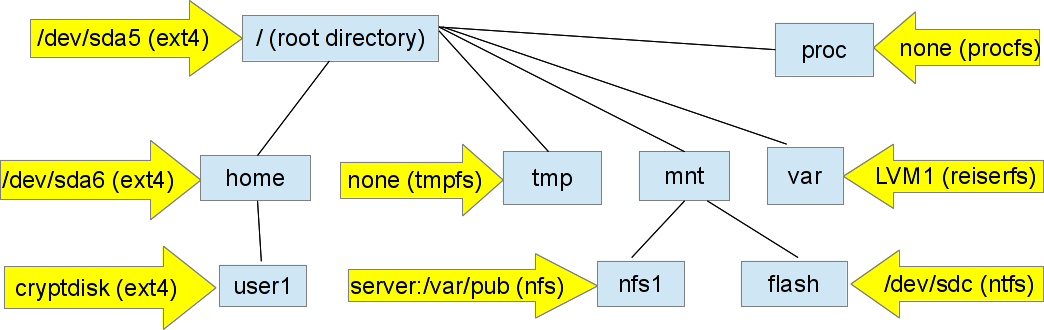
\includegraphics[height=3.5cm]{vfs-and-devices}
\end{frame}

\begin{frame}{Монтирование}
  \begin{itemize}
    \item \alert{Монтирование} - процесс отображения содержимого устройства в указанную папку файловой системы.
    \item Команды:
      \begin{itemize}
        \item монтировать - ( \alert{mount} ) 
        \item размонтировать ( \alert{umount} )
      \end{itemize}
    \item \alert{mount} без параметров - вывести список уже подключенных файловых систем
  \end{itemize}
      \begin{block}{Упражнение. Дерево монтирования.}
     Получить вывод смонтированных блочных устройств в виде дерева с помощью команды: \alert{findmnt}
      \end{block}
  
\end{frame}

}

\mode<all>{\begin{frame}[fragile]{Путь к файлу.}
      \begin{itemize}
        \item Имя файла
                \begin{itemize}
                    \item чувствительно к регистру
                    \item / разделяет директории
                    \item - \textbackslash <Space> специальные символы 
                    \item . скрытый файл
                \end{itemize}
        \item \alert{Полное имя файла} (absolute pathname) начинается с /
        \item \alert{Относительное имя файла} (relative pathname) начинается с
        любого другого символа. Поиск файла производится относительно
        \alert{текущей директории} (current working directory).
      \end{itemize}

      \begin{block}{Примеры}
        ./ - текущая директория

        ../ - предыдущая директория

        ../../usr/bin/ls

        /usr/bin/ls
      \end{block}
\end{frame}

\begin{frame}[fragile]{Навигация по файловой системе}
      \begin{itemize}
		  \item {\tt pwd} -- имя текущей директории (help pwd)
		  \item {\tt ls} -- список файлов в директории. По умолчанию в текущей (man ls)
		  \item {\tt cd} -- смена текущей директории (help cd)
      \end{itemize}
      \begin{block}{Упражнение. Заходим в /usr/bin/ и просматриваем список доступных команд.}
	\begin{lstlisting}
	pwd
	cd /usr/bin/
	pwd
	ls
	cd -	
	pwd
	\end{lstlisting}
      \end{block}
\end{frame}

\begin{frame}[fragile]{Просмотр типов файлов}
      \begin{block}{Упражнение. Символьное обозначение типа файла.}
Первая буква вывода команды ls -l обозначает тип файла. 
Tip. Команды file позволяет определить тип файла. Ключ -d для работы с
директорией. 

/dev/zero

/dev/sda 

.. 

/bin/sh 

/dev/log

/dev/stdout
      \end{block}
\end{frame}

\begin{frame}[fragile]{Команды для работы с файлами}
	\begin{itemize}
		\begin{columns}
		\column{0.2\textwidth}
			\item touch
			\item ln
			\item mkdir
			\item mknod
			\item mkfifo

		\column{0.2\textwidth}
			\item cp
			\item mv
			\item rm
			\item rmdir
			\item file
			\item install

		\column{0.4\textwidth}
			\begin{block}{Упражнение}
				\begin{enumerate}
					\item Создать иерархию директорий
						\begin{lstlisting}
dir1/dir1.1/dir1.1.1
dir1/dir1.2/dir1.2.1
dir1/dir1.2/dir1.2.2
						\end{lstlisting}
					\item Внутри каждой создать файл
					\item Удалить все созданное
				\end{enumerate}
			\end{block}
			
		\end{columns}
	\end{itemize}
\end{frame}
}


\section{ Дополнительные возможности оболочки}
\mode<all>{\input{../../slides/cmdline/bash-intro}}


\begin{frame}{Задание на дом}
\begin{block}{}
vimtutor ru
\end{block}
\end{frame}

\end{document}

